% flashcards-title: Two bounding brackets for a room length compared with a tape-measure reading
% flashcards-desc: A number line marked in meters from three to nine. Above it, one labeled interval bar spans a narrow range near six meters, and a second labeled interval bar spans a wide range from four to eight meters. A dot on the number line marks the later tape-measure reading, labeled six point nine meters.
\documentclass[dvisvgm,tikz,border=8pt]{standalone}
\usepackage{tikz}
\usetikzlibrary{arrows.meta,calc,positioning}
\definecolor{DeckInk}{HTML}{172A3A}
\definecolor{DeckAccent}{HTML}{176B87}
\definecolor{DeckWarm}{HTML}{D97706}
\definecolor{DeckMuted}{HTML}{667784}
\definecolor{DeckPaper}{HTML}{F7FAFC}
\tikzset{
  every node/.style={font=\sffamily, text=DeckInk},
  object/.style={draw=DeckInk, line width=1.1pt, fill=DeckPaper},
  primary/.style={draw=DeckAccent, line width=1.5pt},
  boundary/.style={draw=DeckAccent, line width=1.5pt, dashed, rounded corners=6pt},
  guide/.style={draw=DeckMuted, line width=0.9pt, dashed},
  dimension/.style={{Stealth[length=3.2mm,width=2.2mm]}-{Stealth[length=3.2mm,width=2.2mm]}, draw=DeckWarm, line width=1.2pt},
  motion/.style={-{Stealth[length=3.5mm,width=2.5mm]}, draw=DeckAccent, line width=1.5pt, dashed},
}

\begin{document}
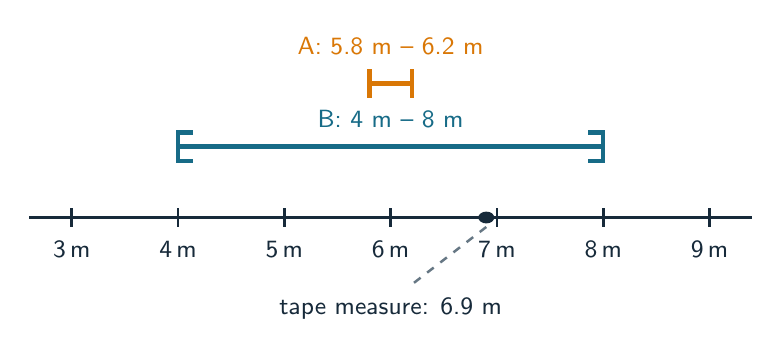
\begin{tikzpicture}[x=1.35cm]
  % Number line with ticks
  \draw[object] (2.6,0) -- (9.4,0);
  \foreach \x in {3,...,9} {
    \draw[DeckInk, line width=1.0pt] (\x,-0.12) -- (\x,0.12);
    \node[below, font=\sffamily\small] at (\x,-0.18) {\x\,m};
  }
  % Bracket A: narrow interval 5.8 to 6.2, flat end caps
  \draw[DeckWarm, line width=1.6pt] (5.8,1.7) -- (6.2,1.7);
  \draw[DeckWarm, line width=1.6pt] (5.8,1.52) -- (5.8,1.88);
  \draw[DeckWarm, line width=1.6pt] (6.2,1.52) -- (6.2,1.88);
  \node[above, font=\sffamily\small, text=DeckWarm] at (6.0,1.95)
    {A: 5.8 m -- 6.2 m};
  % Bracket B: wide interval 4 to 8, square bracket end caps
  \draw[DeckAccent, line width=1.6pt] (4,0.9) -- (8,0.9);
  \draw[DeckAccent, line width=1.6pt] (4.14,0.72) -- (4,0.72) -- (4,1.08) -- (4.14,1.08);
  \draw[DeckAccent, line width=1.6pt] (7.86,0.72) -- (8,0.72) -- (8,1.08) -- (7.86,1.08);
  \node[above, font=\sffamily\small, text=DeckAccent] at (6.0,1.02)
    {B: 4 m -- 8 m};
  % Tape-measure reading on the line
  \fill[DeckInk] (6.9,0) circle (0.075);
  \draw[guide] (6.9,-0.12) -- (6.2,-0.85);
  \node[below, font=\sffamily\small] at (6.0,-0.9) {tape measure: 6.9 m};
\end{tikzpicture}
\end{document}
